\documentclass[handout]{beamer} 
\title{ITCS 532:\\ 
2. Turing Machine Variants}
\date{}
\author{Rob Egrot}

\usepackage{amsmath, bbold, bussproofs,graphicx}
\usepackage{mathrsfs}
\usepackage{amsthm}
\usepackage{amssymb}
\usepackage[all]{xy}
\usepackage{multirow}
\usepackage{tikz-cd}


\newtheorem{proposition}[theorem]{Proposition}
\newcommand{\bN}{\mathbb{N}}
\newcommand{\bZ}{\mathbb{Z}}
\newcommand{\bQ}{\mathbb{Q}}
\newcommand{\bR}{\mathbb{R}}
\newcommand{\bP}{\mathbb{P}}
\newcommand{\tvs}{\textvisiblespace}
\newcommand{\ra}{\rightarrow}
\newcommand{\la}{\leftarrow}

\addtobeamertemplate{navigation symbols}{}{%
    \usebeamerfont{footline}%
    \usebeamercolor[fg]{footline}%
    \hspace{1em}%
    \insertframenumber/\inserttotalframenumber
}
\setbeamertemplate{theorems}[numbered]
\begin{document}

\begin{frame}
\titlepage
\end{frame}

\begin{frame}
\frametitle{Variants of Turing machines}
\begin{itemize}
\item Last class we saw the definition of a Turing machine.
\item This definition is to some extent arbitrary.
\item We could make trivial changes and not affect what can be computed. E.g.
\begin{itemize}
\item No $:$ symbol at start of tape (rules for `hanging' computations).
\item Allow machines to write and move in the same action.
\item Etc.
\end{itemize}
\item We could also make more serious looking changes. E.g.
\begin{itemize}
\item Allow multiple tapes.
\item Allow two-way infinite tapes.
\item Allow infinite states.
\end{itemize}
\item Some of these changes make a significant difference to the computational power of the machine, but others do not.
\item We explore this in this class.
\end{itemize}

\end{frame}

\begin{frame}
\frametitle{Multiple tape Turing machines}
\begin{itemize}
\item A standard Turing machine has only one tape. 
\vspace{0.1cm}
\item We can change the definition so that the machine has two, or even more. 
\vspace{0.1cm}
\item Each tape has its own tape head, but the machine has one global state. 
\vspace{0.1cm}
\item Each tape head works on its tape independently of the others, according to the transition function $\delta$.
\vspace{0.1cm}
\item Question: Should a 2-tape machine be more powerful than a 1-tape machine?
\vspace{0.1cm}
\item I.e. are there decision problems that are solvable by a 2-tape machine that are not solvable by a 1-tape machine (ignoring run time)?
\end{itemize}

\end{frame}

\begin{frame}
\frametitle{Multiple tape Turing machines}
\begin{itemize}
\item Intuitively we might expect that 2-tape machines are more powerful than 1-tape machines. 
\vspace{0.2cm}
\item In other words, that TMs with more than one tape could decide more problems and recognize more languages than their single-tape counterparts. 
\vspace{0.2cm}
\item It turns out that this is \emph{not} the case. 
\vspace{0.2cm}
\item Multi-tape TMs are equivalent to single-tape TMs, in the sense that for any multi-tape TM there's a single-tape TM that gets the same result for the same input.
\vspace{0.2cm}
\item This is not obvious, but we prove it in theorem \ref{T:multi} later.
\end{itemize}

\end{frame}

\begin{frame}
\frametitle{Multiple tape Turing machines - formal definition}
\begin{definition}[$k$-tape Turing machine]
A $k$-tape Turing machine $M_k$ is a modified TM with the following additional properties:
\vspace{0.1cm}
\begin{itemize}
\item $M_k$ has $k$ one-way infinite tapes and $k$ tape heads. 
\vspace{0.1cm}
\item At any moment $M_k$ is in a state $q$. I.e. all tape heads share a single state.
\vspace{0.1cm}
\item We formally describe $M_k$ as a $5$-tuple $(Q,\Sigma,q_0,H,\delta)$.
\begin{equation*}\delta:(Q\setminus H)\times (\Sigma\cup\{\tvs,:\})^k\to Q\times (\Sigma\cup \{\tvs,\la,\ra\})^k\end{equation*}
\item One tape (call it tape 1) is the designated input tape, and all other tapes start blank.
\vspace{0.1cm}
\item Tape 1 is also the output tape.
\end{itemize}
\end{definition}

\end{frame}



\begin{frame}
\frametitle{Two tapes on one}
\begin{theorem}\label{T:multi}
If $\Sigma$ is a finite alphabet and $M$ is a $k$-tape TM using $\Sigma$ there is a finite alphabet $\Sigma'\supseteq\Sigma$ and a single-tape Turing machine $M'$ using $\Sigma'$ such that for all $x\in \Sigma^*$ we have $M(x)=M'(x)$.  
\end{theorem}
\textbf{Proof}
\begin{itemize}
\item The idea is to represent the state of all the tapes, and the positions of all the tape heads, on one tape. 
\item To do this we need to expand the alphabet $\Sigma$. 
\item Before we make a formal definition we'll look at an example with two tapes.
\end{itemize}
\end{frame}

\begin{frame}
\frametitle{Multiple tape Turing machines - equivalence}
\[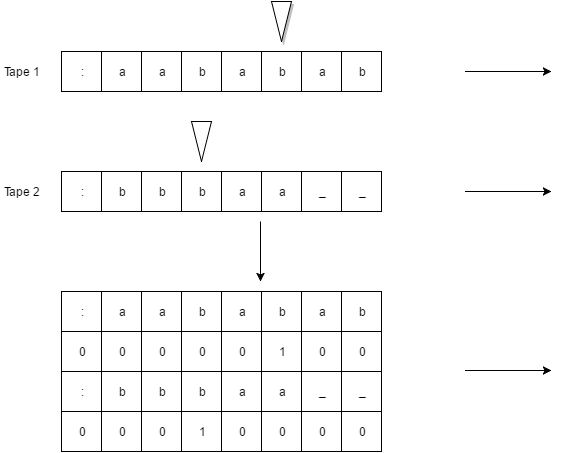
\includegraphics[scale = 0.5]{dMulti.png}\]  
\end{frame}

\begin{frame}
\frametitle{Extending the alphabet}
\begin{itemize}
\item We want to define an extended alphabet $\Sigma'$.
\vspace{0.1cm}
\item In any square other than the first (which is a special case as only $:$ can be written there on each tape), there are $|\Sigma\cup\{\tvs\}|$ possibilities for each tape.
\vspace{0.1cm}
\item Also for each tape the tape head may or not be present. 
\vspace{0.1cm}
\item So we need $(|\Sigma|+1)^k\times 2^k$ symbols to cover all these possible combinations. 
\vspace{0.1cm}
\item In addition we need $2^k$ extra symbols for the first squares of the tapes (where only $:$ can be written but the tape head may or may not be present). 
\vspace{0.1cm}
\item Finally we also need every symbol from $\Sigma$ (so that $\Sigma\subset \Sigma'$). 
\vspace{0.1cm}
\item So we need $((|\Sigma|+1)^k+1)\times 2^k+|\Sigma|$ symbols in $\Sigma'$.
\end{itemize}

\end{frame}

\begin{frame}
\frametitle{Defining $M'$}
\begin{itemize}
\item Remember we start with multi-tape $M$, and we want to define single tape $M'$ that does the same thing.
\vspace{0.1cm}
\item We describe the operation of $M'$ step by step.
\vspace{0.1cm}
\item We assume two tapes, as general idea is the same.
\end{itemize}
\begin{enumerate}
\item $M'$ scans the input $x$ and rewrites $x$ using composite symbols. E.g. $aba\tvs$ will become 
\[ \begin{array}{cccc}
: & a & b & a  \\
1 & 0 & 0 & 0 \\
: & \tvs & \tvs & \tvs  \\
1 & 0 & 0 & 0  
\end{array} \] 
The tape of  $M'$ now represents the initial configuration of $M$ with input $x$. 
\end{enumerate} 
\end{frame}

\begin{frame}
\frametitle{Defining $M'$}
\begin{enumerate}
\item[2.] 
\begin{itemize}
\item $M'$ scans the tape till it finds the 1 representing the position of the first tape head. 
\vspace{0.1cm}
\item $M'$ changes state to record the symbol the 1st tape head would be reading. 
\vspace{0.3cm}
\end{itemize}
\item[3.] 
\begin{itemize}
\item $M'$ scans the tape for the 1 representing the position of the 2nd tape head.
\vspace{0.1cm}
\item $M'$ changes state to record what symbols the tape heads of $M$ are reading.
\end{itemize} 
\vspace{0.1cm}
\end{enumerate} 
($M'$ needs many more states that $M$, as it must record the configuration of $M$ in its state). 
\end{frame}

\begin{frame}
\frametitle{Defining the $M'$}
\begin{enumerate}

\item[4.] Based on the recorded information about the current symbols being read and the simulated state of $M$ (which $M'$ stores via its own state), $M'$ rewrites the tape to represent $M$ acting on all its tapes.
\vspace{0.2cm}
\item[5.] Steps 2, 3, and 4 repeat till $M$ would enter a halting state (if this ever happens!), at which point we proceed to either 6 or 7, depending on the kind of halting state:
\vspace{0.2cm}
\item[6.] (Acceptance) $M'$ rewrites the tape so that the output as written on the top row of the combined tape is now written using symbols from $\Sigma$ (so it matches the output of $M$). 
\vspace{0.2cm}
\item[7.] (Rejection) $M'$ enters a rejection state.
\end{enumerate} 
\end{frame}

\begin{frame}
\frametitle{Defining $M'$}
\begin{itemize}
\item $M'$ is equivalent to $M$.
\vspace{0.4cm}
\item I.e. Given input $x$, $M'$ accepts/rejects iff $M$ accepts/rejects, and the output is the same.
\vspace{0.4cm}
\item This completes the proof.
\vspace{0.4cm}
\item Question: Why is it easy to model a single-tape TM using a multi-tape machine?
\end{itemize}

\end{frame}

\begin{frame}
\frametitle{Two-way infinite tapes}
\begin{itemize}
\item The tape of a regular TM is only infinite in one direction.
\vspace{0.2cm} 
\item What if we modified the definition to allow the tape to be infinite in both directions? 
\vspace{0.2cm}
\item Would this be a more powerful model of computation? It turns out no. 
\vspace{0.2cm}
\item Think about the multi-tape example. 
\vspace{0.2cm}
\item A two-way infinite tape with only one head is at most as powerful as a TM with two tapes and two tape heads. 
\vspace{0.2cm}
\item But we saw that this has the same power as a regular TM. 
\vspace{0.2cm}
\item Since a TM with a two-way infinite tape is certainly not \emph{less} powerful than a regular TM, they must be equivalent. 
\end{itemize}

\end{frame}

\begin{frame}
\frametitle{More than one tape head}
\begin{itemize}
\item We could modify the definition of a Turing machine so that there are two (or more) tape heads working on the same tape. 
\item This is slightly tricky to formally define because we have to deal with the possibility of `simultaneous edits'.
\item  It turns out we can simulate a multi-head TM using a regular TM like how we simulated the multi-tape TM. 
\item I.e. add symbols to the language to model the tape and the positions of the tape heads on a single tape:
\[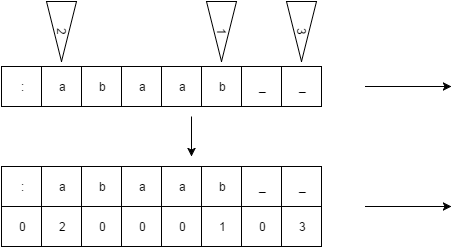
\includegraphics[scale = 0.5]{dMH.png} \]  
\end{itemize}

\end{frame}

\begin{frame}
\frametitle{Grid instead of tape}
\begin{itemize}
\item How about instead of a tape we have an infinite grid that the tape head moves around on in two dimensions? 
\vspace{0.2cm}
\item Again this is not more powerful. 
\vspace{0.2cm}
\item To see this we first model the 2D grid as a sequence of squares in one dimension. 
\vspace{0.2cm}
\item This is similar to how we showed the rational numbers are countable. 
\vspace{0.2cm}
\item Then we have to create enough states and design the code well enough to deal with the fact that moving the tape head is more complicated now. 
\vspace{0.2cm}
\item It's tricky but it can be done.
\vspace{0.2cm}
\item Question: Why are the rational numbers countable?
\end{itemize}

\end{frame}

\begin{frame}
\frametitle{$\mathbb{Q}$ is countable}
\[\xymatrix{ 
\bullet_{(0,4)} & \bullet_{(1,4)}\ar@{.>}[dr] & \bullet_{(2,4)} & \bullet_{(3,4)}\ar@{.>}[dr] & \bullet_{(4,4)}\\
\bullet_{(0,3)}\ar@{.>}[dr]  & \bullet_{(1,3)}\ar@{.>}[ul] & \bullet_{(2,3)}\ar@{.>}[dr]  & \bullet_{(3,3)}\ar@{.>}[ul] & \bullet_{(4,3)} \\
\bullet_{(0,2)}\ar@{.>}[u]  & \bullet_{(1,2)}\ar@{.>}[dr]  & \bullet_{(2,2)}\ar@{.>}[ul] & \bullet_{(3,2)}\ar@{.>}[dr]  & \bullet_{(4,2)}\ar@{.>}[ul]  \\
\bullet_{(0,1)}\ar@{.>}[dr]  & \bullet_{(1,1)}\ar@{.>}[ul]  & \bullet_{(2,1)}\ar@{.>}[dr]  & \bullet_{(2,1)}\ar@{.>}[ul] & \bullet_{(4,1)} \\
\bullet_{(0,0)}\ar@{.>}[u] & \bullet_{(1,0)}\ar@{.>}[r]  & \bullet_{(2,0)}\ar@{.>}[ul] & \bullet_{(3,0)}\ar@{.>}[r]  & \bullet_{(4,0)}\ar@{.>}[ul]  }\]
\end{frame}

\begin{frame}
\frametitle{Infinite states}
\begin{itemize}
\item Regular Turing machines can only have a finite number of states.
\vspace{0.1cm} 
\item How about if we allow the machine to have an infinite number of states? 
\vspace{0.1cm}
\item This is more powerful! 
\vspace{0.1cm}
\item In fact it's too powerful. 
\vspace{0.1cm}
\item If we're allowed to use an infinite number of states then every language over a countable alphabet can be decided by a TM. 
\vspace{0.1cm}
\item This is because with an infinite number of states we can have one unique state for every possible input. 
\vspace{0.1cm}
\item So all we have to do to `decide' a language is assign acceptance or rejection to each state appropriately. 
\vspace{0.1cm}
\item Having an infinite number of states is more like magic than computation.  
\end{itemize}

\end{frame}

\begin{frame}
\frametitle{The Church-Turing Thesis}
\begin{centering} \textbf{The Church-Turing Thesis}

\emph{Any problem expressible in a formal language that is solvable by a well-defined step by step procedure can be solved by a Turing machine} \end{centering}
\newline
\begin{itemize}
\item `Thesis' here is used to mean ``A statement or theory". 
\vspace{0.2cm}
\item It's impossible to formally prove the Church-Turing thesis, but it would be theoretically possible to disprove it by producing a counterexample.
\begin{itemize}
\vspace{0.2cm}
\item Though how would you check that your step by step procedure for this hypothetical problem was correct?
\end{itemize}
\vspace{0.2cm}
\item Most computer scientists believe the Church-Turing thesis.
\vspace{0.2cm}
\item So we use the theory of Turing machines to put hard theoretical limits on computation.
\end{itemize}
\end{frame}

\begin{frame}
\frametitle{Enumerators}
\begin{itemize}
\item Recall that a formal language $L$ is defined to be recursively enumerable if there is a Turing machine that accepts when given words from $L$ as input, and does not halt for other inputs. 
\vspace{0.2cm}
\item \emph{Enumerable} in English means `can be counted'.
\vspace{0.2cm}
\item  So a \emph{recursively enumerable} language should, logically, be one that can be counted (put into a list) by a recursive procedure. 
\vspace{0.2cm}
\item But the standard definition of an r.e. language doesn't say anything about lists or counting.
\vspace{0.2cm}
\item What is going on? 
\vspace{0.2cm}
\item It turns out that these definitions are equivalent, in a way we make precise now.
\end{itemize}

\end{frame}

\begin{frame}
\frametitle{Enumerators - formal definition}
\begin{definition}[Enumerator]
An enumerator is a special Turing machine with the following properties:
\begin{enumerate}
\item There is no halt state.
\item There is a special state \emph{print}.
\item The machine starts by erasing the input (or we just assume the input is always empty).
\item When the machine enters the \emph{print} state the current contents of the tape between $:$ and the first $\tvs$ is `printed' (added to the end of an abstract list that starts empty).
\end{enumerate}
\end{definition} 
\end{frame}

\begin{frame}
\frametitle{Enumerators and formal languages}
\begin{itemize}
\item Enumerators capture the intuitive idea of generating a list using an automated procedure. 
\vspace{0.2cm}
\item Given a finite alphabet $\Sigma$, and an enumerator $E$ using $\Sigma$, the set of words that will eventually be printed by $E$ form a subset of $\Sigma^*$.
\vspace{0.2cm}
\item I.e. it's a formal language. 
\vspace{0.2cm}
\item It turns out that every language created using an enumerator is r.e., and every r.e. language has an enumerator that generates it. 
\vspace{0.2cm}
\item This is not obvious, so we prove it as theorem \ref{T:enum} now.
\end{itemize}
\end{frame}

\begin{frame}
\frametitle{Enumerators and formal languages}
\begin{theorem}\label{T:enum}
Let $\Sigma$ be a finite alphabet and let $L\subseteq\Sigma^*$. Then $L$ is recursively enumerable if and only if there is an enumerator $E$ with the following properties:
\vspace{0.2cm}
\begin{enumerate}
\item If $s\in L$ then $E$ will print $s$ after a finite number of operations.
\vspace{0.2cm}
\item If $E$ prints $s$ then $s\in L$.
\end{enumerate}
\end{theorem}

\end{frame}

\begin{frame}
\frametitle{Proof: has enumerator implies r.e.}
\begin{itemize}
\item We start by proving that if an enumerator $E$ exists for $L$ then $L$ is r.e. as this is relatively easy. 
\vspace{0.2cm}
\item We use enumerator $E$ to build a Turing machine $T_E$ that accepts for all words in $L$, and fails to halt for all other words.
\vspace{0.2cm}
\item By theorem \ref{T:multi} we can assume that $T_E$ has multiple tapes.
\vspace{0.2cm}
\item $T_E$ stores the input string on one tape, and on another tape it outputs strings as produced by $E$. 
\vspace{0.2cm}
\item Every time a new string is produced, $T_E$ compares it to the input string.
\vspace{0.2cm} 
\item If they are the same it accepts. 
\vspace{0.2cm}
\item Since $E$ is an enumerator for $L$, if the input string is in $L$ it will eventually be produced by $E$. 
\vspace{0.2cm}
\item So $T_E$ semidecides $L$ as required.
\end{itemize}
\end{frame}

\begin{frame}
\frametitle{Proof: r.e. implies has enumerator}
\begin{itemize}
\item Harder. Suppose $T$ semidecides $L$.
\vspace{0.2cm}
\item We want to use this to create an enumerator $E_T$ that lists the elements of $L$. 
\vspace{0.2cm}
\item Idea: $E_T$ will write the strings from $\Sigma^*$ one by one on a tape (again we can safely assume multiple tapes). 
\vspace{0.2cm}
\item Every time a new string is written $E_T$ runs $T$ on that string. If $T$ accepts then $E_T$ `prints' the string. So the flow would be something like this:
\end{itemize}
\[\includegraphics[scale = 0.3]{dEnum.png} \]  
\end{frame}

\begin{frame}
\frametitle{Proof: r.e. implies has enumerator}
\begin{itemize}
\item Problem. $T(x)$ may not halt! So as soon as we get a string not in $L$ our machine $E_T$ will get stuck and will run forever without printing again. 
\item We use \emph{dovetailing} to solve this. The modified action of $E_T$ is as follows
\begin{enumerate}
\item Generate a new string $x_1$.
\item Simulate $T(x_1)$ for one step only.
\item Generate a new string $x_2$.
\item Simulate $T(x_1)$ for one more step, then simulate $T(x_2)$ for one step.
\item Generate a new string $x_3$.
\item Simulate $T(x_1)$ for one more step, then simulate $T(x_2)$ for one more step, then simulate $T(x_3)$ for one step.
\item And so on...
\item Whenever $T(x_n)$ succeeds print $x_n$. 
\end{enumerate}
\end{itemize} 
\end{frame}

\begin{frame}
\frametitle{Proof: r.e. implies has enumerator}
\begin{itemize}
\item This works because even if one or more of the computations never halts it doesn't matter. 
\vspace{0.2cm}
\item Because we add an extra string every cycle, the strings that $T$ doesn't accept don't stop the other strings from getting attention. 
\vspace{0.2cm}
\item Again this is similar to the argument proving $\mathbb{Q}$ is countable.
\vspace{0.2cm}
\item We know that, for all values of $x$, we will eventually have simulated $T(x)$ for any given number of steps. 
\vspace{0.2cm}
\item It might take a long time, but if $T$ accepts $x$ then $E_T$ will notice and print $x$. 
\vspace{0.2cm}
\item We have to manage all this using Turing machine architecture, but we have lots of tapes at our disposal.
\end{itemize} 
\end{frame}



\end{document}